\section{Билет 35. Термодинамика. Термодинамическая система. Термодинамические параметры. Состояние термодинамической системы. Термодинамический процесс. Температура, абсолютная шкала температур Кельвина.}

\begin{definition}
\textbf{Термодинамикой} называется раздел физики, изучающий общие свойства макроскопических систем, находящихся в состоянии термодинамического равновесия, и процессы перехода между этими состояниями. В отличие от молекулярно-кинетической теории, термодинамика не рассматривает микроскопическую картину процессов, а базируется на нескольких фундаментальных законах (началах термодинамики), установленных на основе обобщения опытных фактов.
\end{definition}

\begin{definition}
\textbf{Термодинамической системой} называется совокупность макроскопических тел, выделенных для исследования и обменивающихся энергией и/или веществом с окружающей средой или между собой.
Физические величины, характеризующие состояние системы, называются \textbf{термодинамическими параметрами}. К основным макроскопическим параметрам относятся:
\begin{itemize}
    \item Давление $p$ (Па);
    \item Объём $V$ (м³);
    \item Температура $T$ (К);
    \item Масса $m$ или количество вещества $\nu$ (моль).
\end{itemize}
\end{definition}

\begin{definition}
\textbf{Равновесным состоянием} системы называется такое состояние, при котором все параметры системы имеют определённые значения, остающиеся при неизменных внешних условиях постоянными сколь угодно долго.
Если хотя бы один параметр не имеет определённого значения (например, температура в разных точках тела различна), состояние называется \textbf{неравновесным}. Процесс самопроизвольного перехода системы из неравновесного состояния в равновесное называется \textbf{релаксацией}, а время, за которое отклонение параметра от равновесного значения уменьшается в $e$ раз, --- \textbf{временем релаксации}.
\end{definition}

\begin{definition}
\textbf{Термодинамическим процессом} называется переход системы из одного равновесного состояния в другое.
\begin{itemize}
    \item Процесс, состоящий из непрерывной последовательности равновесных состояний, называется \textbf{равновесным (квазистатическим)}. Он может быть проведён в обратном направлении, поэтому такие процессы называют \textbf{обратимыми}.
    \item Процесс, при котором система после ряда изменений возвращается в исходное состояние, называется \textbf{круговым процессом} или \textbf{циклом}.
\end{itemize}
\end{definition}

\begin{remark}
\textbf{Температура и шкала Кельвина.} Температура --- макроскопический параметр, характеризующий состояние теплового равновесия системы. При тепловом контакте двух тел происходит обмен энергией до тех пор, пока их температуры не станут равными.
\par\noindent В СИ единицей температуры является \textbf{кельвин (К)}. Абсолютная термодинамическая шкала Кельвина строится так, что нулевая точка соответствует \textbf{абсолютному нулю} ($-273.15\,^\circ\text{C}$), при котором прекращается тепловое движение молекул в классическом приближении.
\par\noindent Связь между абсолютной температурой $T$ и температурой по шкале Цельсия $t$:
\begin{equation}
    T = t + 273.15 \quad \text{[К]}. \label{eq:temp_scale_35}
\end{equation}
Разность температур в кельвинах равна разности в градусах Цельсия: $\Delta T = \Delta t$.
\end{remark}

\begin{figure}[H]
\centering
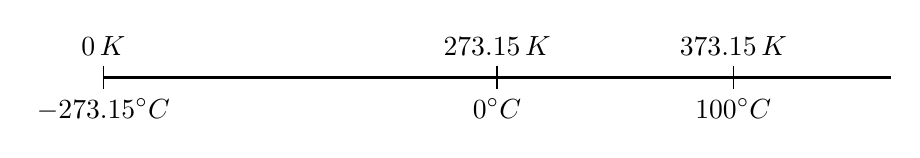
\begin{tikzpicture}

\draw[thick] (0,0)--(10,0);

\foreach \x in {0,5,8}
{
\draw (\x,0.15)--(\x,-0.15);
}

\node[above] at (0,0.15) {$0\,K$};
\node[above] at (5,0.15) {$273.15\,K$};
\node[above] at (8,0.15) {$373.15\,K$};

\node[below] at (0,-0.15) {$-273.15^\circ C$};
\node[below] at (5,-0.15) {$0^\circ C$};
\node[below] at (8,-0.15) {$100^\circ C$};

\end{tikzpicture}
\caption{Соответствие шкал Кельвина и Цельсия.}
\end{figure}
